\chapter{Atoms and Elements}

\section{History}
\begin{description}
  \item[Democritus] thought that all things are made of indivisible bits
  \item[Aristotle] disagreed with the idea of the atom and muted discussion
\end{description}

\section{Basic Laws}
\begin{description}
  \item[The Law of Conservation of Mass] matter is neither created nor destroyed
    during ordinary chemical and physical changes.
  \item[The Law of Definite Proportions] chemical compounds have the same
    elements in the same proportions by mass regardless of the size of the
    sample
  \item[The Law of Multiple Proportions] when chemical elements combine they
    will do so in small, whole-number rations.  If two elements can form
    multiple compounds, the ratio of the second element to a fixed mass of the
    1st element will always be a small, fixed number.
\end{description}

\section{Dalton's Atomic Theory}
\begin{enumerate}
  \item All mater is composed of atoms
  \item Atoms of an element are identical, atoms of different elements are
    dissimilar in proportions
  \item Atoms cannot be subdivided, created, or changed
  \item Atoms of different elements combine in simple whole number ratios to
    form chemical compounds
  \item In chemical reactions, atoms are combined, seperated or rearranged
\end{enumerate}

\section{Modern Atomic Theory}
\subsection{Universal Truths}
\begin{itemize}
  \item Conservation of mass is obeyed during chemical reactions
  \item All mater is composed soley of atoms
  \item Atoms of any one element differ in proportions from others
\end{itemize}
\subsection{Variations on Dalton's Theory}
\begin{itemize}
  \item Atoms of a type can have different masses (isotopes)
  \item Atoms have an internal structure composed of protons, neutrons, and
    electrons
  \item Atoms can be created and destroyed, but only during nuclear reactions
\end{itemize}

\section{Modern Structure of an Atom}
An atom is the smallest unit of a element which still retains the properties of
that element.

\begin{figure}[H]
  \centering
  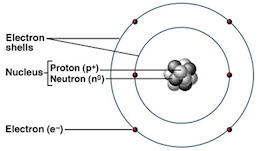
\includegraphics{res/atom_structure.jpg}
  \caption{Modern-day structure of an atom (basic)}
\end{figure}

There are three components that make up the important parts of an atom.  They
are described below:

\begin{description}
  \item[Nucleus] The center of the atom.  Very small, and very dense.  Contains
    protons and neutrons.
    \begin{description}
      \item[Protons] positively charged sub-atomic particles
      \item[Neutrons] neutrally charged sub-atomic particles
    \end{description}
  \item[Electrons] Small, negatively-charged particles.  They orbit the nucleus
    in \textit{electron clouds}.  That is to say that we do not know the
    definite position of an electron, but we can reason about where it is likely
    to be.
\end{description}

\section{Experiments}
\subsection{Cathode Ray Tube}
Experiment preformed by J.J. Thompson.  Contributed first to the discovery of a
sub-atomic particle (the electron).  Showed that a cathode-ray had negatively
charged particles because it responded to magnetic fields.

\begin{figure}[H]
  \centering
  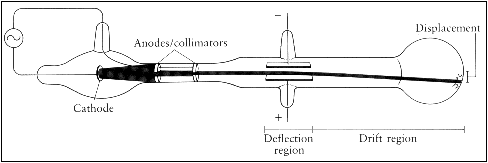
\includegraphics{res/crt_experiment.png}
  \caption{Diagram of the cathode-ray tube expirement.}
\end{figure}

\subsection{Milikan Oil Drop}
Determined the more specific charge of the electron.  Showed that small
particles were able to be suspended when they picked up negative charge.  Using
the charge of the plates involved, the charge was able to be determined.

\begin{figure}[H]
  \centering
  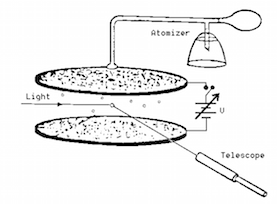
\includegraphics{res/oil_drop_experiment.png}
  \caption{Diagram of the oil-drop experiment.}
\end{figure}

\subsection{Rutherford's Gold Foil}
Experiment preformed by Rutherford and Geiger.  Together, the two of them shot
\textit{alpha} particles at a ultra-thin sheet of gold foil.  These particles
exhibited one of three behaviors, each indicating a different outcome.

\begin{figure}[H]
  \centering
  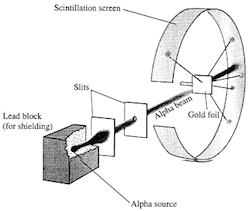
\includegraphics{res/rutherford_exp.png}
  \caption{Diagram of Rutherford's Gold Foil experiment.}
\end{figure}

\begin{description}
  \item[Through the foil] the alpha particles went through empty space within an
    atom, and thus traveled uninterrupted through the atom in a straight path
  \item[Deflected through the foil] the alpha particles were attracted to
    something while traveling through an empty space within the atom.  As such,
    their path was changed slightly, and they angled as they travelled.
  \item[Bounced off the foil] the alpha particles collided with the positively
    charged nucleus to deflect off of the foil, back at the particle gun.
\end{description}

\section{Elements}
Elements are defined by the number of protons in the nucleus of one of their
atoms.  No two elements will ever have the same number of protons in their
nucleus under normal circumstances.  \textit{As such, the number of protons in
an element can be considered as its unique key.}

The atomic number of an element has the same value as the number of protons in
its nucleus.

\subsection{Isotopes}
Isotopes have the same number of protons, but a different number of neutrons.
Isotopes are represented as the following \ce{^{35}_{17}Cl}.  This is
Chlorine-35.  The superscript represents the atomic mass of an isotope, and the
subscript represents the atomic number.

Since the atomic mass is the sum of the number of protons and the number of
neutrons in an atom, the number of neutrons in an isotope can easily be
determined.

\section{Nomenclature}
\subsection{Common Nomenclature}
\begin{description}
  \item[Molecular Compounds] compounds which contain only non-metal components
  \item[Binary Compounds] compounds of two different elements.  In non-ionic
    binary compounds, simply change the last component to have an \textit{-ide}
    suffix, for example \ce{CaCl2} - \textit{Calcium Chloride}.  Naming occurs
    in the order \textit{mono-, di-, tri-, tetra-, penta-, hexa-, hepta-, octa-,
    nona-, deca-}.
  \item[Binary Ionic Compounds] binary-compounds (see above) which contain both
    a metal and a non-metal.
    \begin{enumerate}
      \item Positive charge first
      \item The positive element undergoes no change in the name of its element
      \item Negative charge gets the \textit{-ide} treatment
    \end{enumerate}
\end{description}

\subsection{Stock-system Nomenclature}
When dealing with ions, it is frequently the case where there are more than one
charge state available to work with.  The stock-system nomenclature makes it
obvious which one we are dealing with.

Simply put, you take the charge of an ion, and place it in parenthesis in
roman-numerals to the right of the chemical symbol.  For example, \ce{Fe^3+}
becomes \ce{Fe(III)}.

\section{Types of Ions}
Ions take shape in several different types, but come in only two charges.  These
charges are named \textit{cation} and \textit{anion}.  A cation is a positively
charged ion, whereas an anion is a negatively charged ion.  \textit{(Remember:
a-negative-ion\dots an-ion.)}

\subsection{Monatomic Ions}
Monatomic ions are formed of one ore more of the same kind of element.  These
ions gain and loose electrons to obtain a full valence-level of electrons for
wahtever level they might be at.  Examples include \ce{H^+} and \ce{O^{2-}}.

\subsection{Polyatomic Ions}
Polyatomic ions are charged groups of covalently bonded atoms.  They carry
charge as a group, such that they behave like single ions, even though they are
composed of more than one atom.

All relevant polyatomic ions are listed below, grouped by charge.

\begin{itemize}
  \item Cation\textsuperscript{1+}
    \begin{description}
      \item[Ammonium] \ce{NH4^+}
      \item[Hydronium] \ce{H30^+}
    \end{description}
  \item Anion\textsuperscript{1-}
    \begin{description}
      \item[Cyanide] \ce{CN^-}
      \item[Bicarbonate] \ce{HCO3^-}
      \item[Hydroxide] \ce{OH^-}
      \item[Nitrate] \ce{NO3^-}
      \item[Nitrite] \ce{NO2^-}
      \item[Permanganate] \ce{MnO4^-}
      \item[Acetate] \ce{CH3COO^-} or \ce{C2H3O2^-}
      \item[Dihydrogen Phospate] \ce{H2PO4^-}
    \end{description}
  \item Anion\textsuperscript{2-}
    \begin{description}
      \item[Carbonate] \ce{CO3^2-}
      \item[Sulfate] \ce{SO4^2-}
      \item[Sulfite] \ce{SO3^2-}
    \end{description}
  \item Anion\textsuperscript{3-}
    \begin{description}
      \item[Phosphate] \ce{PO4^3-}
    \end{description}
\end{itemize}
